\section{Exploratory Data Analysis}

\subsection{Data Semantics}
The ATLAS Higgs dataset from the CERN Open data portal has a total of 800K collision events which have been simulated by the high energy ATLAS simulator. The simulator encompasses the current best understanding of the physics underlying the signal and background decays. The signal events mimic properties of the background events as is known to happen in real events. All the events are labelled - either $s$ or $b$ which enable supervised learning techniques to be employed on the data. 

For simplicity, ATLAS uses only three sources of background in creating this particular dataset. Information on the source of each background process is not provided in the dataset. The most abundant background source comes from the decay of the $Z$ boson to two taus. The $Z$ has a mass (91.2 Gev) very close to that of the Higgs (125 Gev) and $Z$ decay occurs much more frequently than the Higgs decay. 

The events are broken up into three categories to facilitate the learning task. The learning task comprises of training, cross-validation and testing and there can be no leakage of data from one group to the other. For this thesis we use the ATLAS proposed division of the data. The density of events in each of the three individual sets in highlighted in table \ref{break}.
This is to aid in analysis of the data and prevent users from splitting the data into training and test sets in a way that distorts the density of signal events by over-sampling or under-sampling.  

\begin{table}[H]
\begin{center}
\begin{tabular}{l|c|c|c}
Dataset & Total events & Background $|\mathcal{B}|$ &  Signal $|\mathcal{S}|$ \\
\toprule
Training & 250,000 & 164,333 & 85,667 \\
Cross Validation & 100,000 & 65,975 & 34,025\\
Testing & 450,000 & 296,317 & 153,683\\

\end{tabular}
\caption{ATLAS Breakdown of datasets for the learning task}
\label{break}
\end{center}
\end{table}
Some of the feature values in the dataset have the tag -999.0. They cannot exactly be termed as missing data since data is structurally absent in these cases and cannot be computed. For instance, data with PRI$\_$jet$\_$num = 0 means the collision event did not produce any jets, this implies that such events also do not have any of the features based on jet properties. In a similar fashion, there are features which are structurally undefined for several events. The fraction of events undefined for each feature and class are summarized in the table below: 
 
\begin{table}[H]
%\resizebox{\textwidth}{!}{
\begin{tabular}{l|c|c|c}
Feature & Background undefined & Signal undefined & Total undefined\\
\toprule
PRI$\_$tau$\_$pt &  - & - & \rdelim\}{10}{20pt}[\parbox{12.5mm}{None}] \\
PRI$\_$tau$\_$eta & - & - & \\
PRI$\_$tau$\_$phi & - & - & \\ 
PRI$\_$lep$\_$pt & - & - & \\
PRI$\_$lep$\_$eta & - & - & \\
PRI$\_$lep$\_$phi & - & - & \\
PRI$\_$met & - & - & \\
PRI$\_$met$\_$sumet & - & - & \\
PRI$\_$met$\_$phi & - & - & \\
PRI$\_$jet$\_$num & - & - & \\
\midrule
PRI$\_$jet$\_$leading$\_$pt & \rdelim\}{3}{20pt}[30$\%$] & \rdelim\}{3}{20pt}[10$\%$] & \rdelim\}{3}{20pt}[40$\%$]\\ 
PRI$\_$jet$\_$leading$\_$eta & & & \\
PRI$\_$jet$\_$leading$\_$phi & & & \\
\midrule
PRI$\_$jet$\_$subleading$\_$pt & \rdelim\}{3}{20pt}[50$\%$] & \rdelim\}{3}{20pt}[21$\%$]  & \rdelim\}{3}{20pt}[71$\%$] \\
PRI$\_$jet$\_$subleading$\_$eta & & & \\
PRI$\_$jet$\_$subleading$\_$phi &  & & \\
\midrule
PRI$\_$jet$\_$all$\_$pt & - & - & - \\
\midrule
DER$\_$mass$\_$MMC & 14$\%$ & 1$\%$ & 15$\%$ \\
\midrule
DER$\_$mass$\_$transverse & - & - & \rdelim\}{3}{20pt}[\parbox{12.5mm}{None}] \\
DER$\_$mass$\_$vis & - & - & \\
DER$\_$pt$\_$h & - & - & \\
\midrule
DER$\_$deltaeta$\_$jet$\_$jet & \rdelim\}{4}{20pt}[50$\%$] & \rdelim\}{4}{20pt}[21$\%$]  & \rdelim\}{4}{20pt}[71$\%$] \\
DER$\_$mass$\_$jet$\_$jet & & & \\
DER$\_$prodeta$\_$jet$\_$jet & & & \\
DER$\_$lep$\_$eta$\_$centrality & & & \\
\midrule
DER$\_$deltar$\_$tau$\_$lep & & & \rdelim\}{5}{20pt}[\parbox{12.5mm}{None}] \\
DER$\_$pt$\_$tot & - & - & \\
DER$\_$sum$\_$pt & - & - & \\
DER$\_$pt$\_$ratio$\_$lep$\_$tau & - & - & \\
DER$\_$met$\_$phi$\_$centrality & - & - & \\
\midrule
\end{tabular}
\caption{Fraction of undefined values in the ATLAS Higgs dataset}
\label{missing_values}
\end{table}

It is important to point out that almost all undefined features are related to \texttt{PRI$\_$jet$\_$num} = 0 except \texttt{DER$\_$mass$\_$MMC}. From the table we gauge that 40$\%$ of events had no jets and hence no leading jet properties and 71$\%$ of events had less than 2 jets (atleast 2 jets are needed for subleading jet properties). Ignoring events which have an undefined tag in any of the features gets rid of a large number of events. For instance, more than 62$\%$ of the signal events lack atleast one feature, hence we need to work with events that have missing values.  

Traditionally, missing values are imputed with either the mean or the median to bring the data-point back to into the normal range of values. However, such imputation creates artificial peaks in the distribution of the features and it is important to verify it does not distort classification performance. For features with skewed distributions, the median is a better imputer than mean as the median is more robust to outliers. 

Each event in the dataset has an importance weight $w_{i}$, they were introduced in chapter \ref{formal} (see eq. \ref{wratio}). The weight for a signal event is on average 300 times smaller than the weight for a background event. Due to this, weights cannot be used as features as their magnitude can predict signal and background events perfectly. However, they do form a part of the training process but not as a non-traditional feature.

\begin{figure}[H]
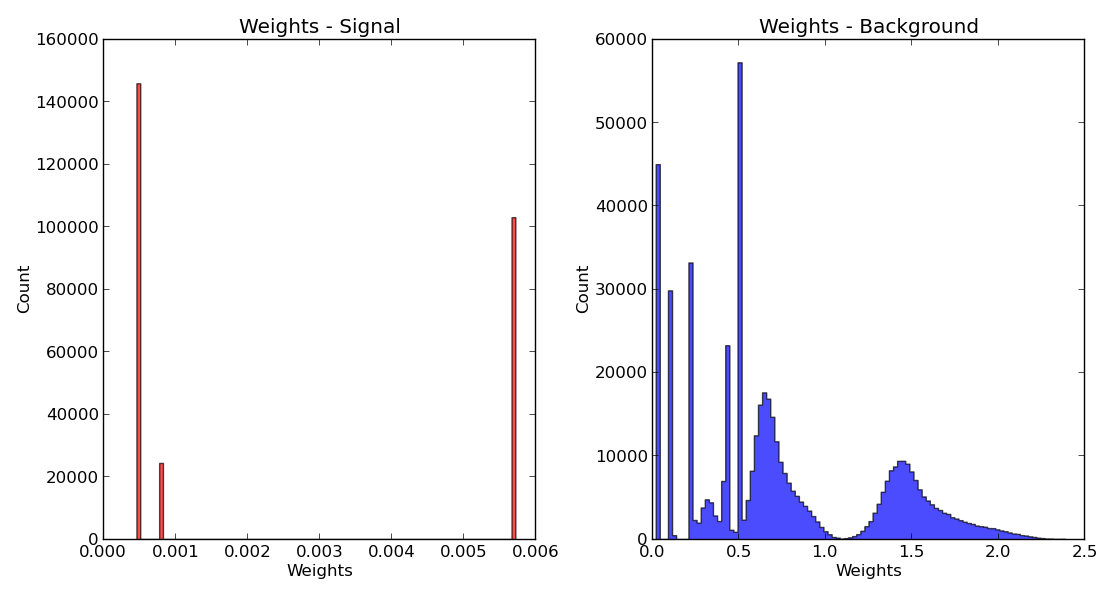
\includegraphics[scale=0.5]{images/weights.png}
\caption{Distribution of weights of the signal and background class}
\label{weightsd}
\end{figure}

Fig. \ref{weightsd} depicts the distribution of weights across the whole dataset for signal and background classes. The peaks in the background weight distribution correspond to the individual sources of background events used by the simulator. In the weight distribution for signals we see 3 distinct spikes, they indicate Higgs production by 3 unique mechanisms. Apart from the weights there is no information in the dataset to indicate the specific signal mechanism or background source. 

\subsection{Features}

ATLAS provides 30 features for each signal and background event in the dataset. These features were described section \ref{features}. The features are partitioned into primary and derived features. The derived features are more discriminatory than the primary features as the former represent quantities calibrated by physicists while the latter are raw momenta of particles observed in the decay channel. In fig. \ref{unscaled_features1} and \ref{unscaled_features2} we depict the distributions of derived features split by signal and background events.

\begin{figure}
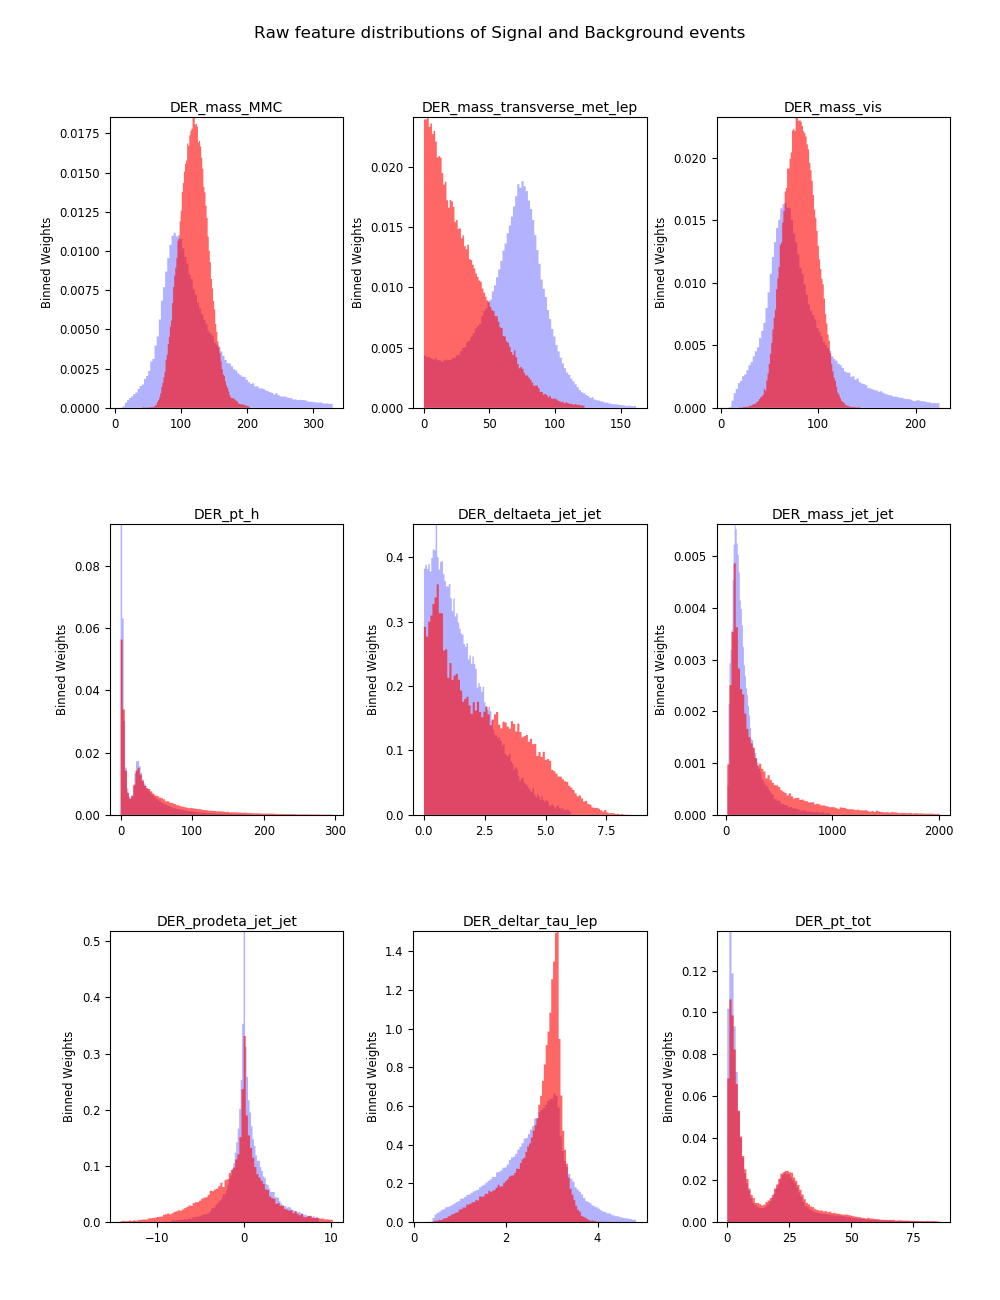
\includegraphics[width=\textwidth]{images/der_features1.png}
\caption[Raw feature distributions]{Raw feature distributions of signal (red) and background (blue) events depicting values on their true scale, further in order to make the histogram more representative we sum importance weights $w_{i}$ in each bin rather than count.}
\label{unscaled_features1}
\end{figure}

\begin{figure}
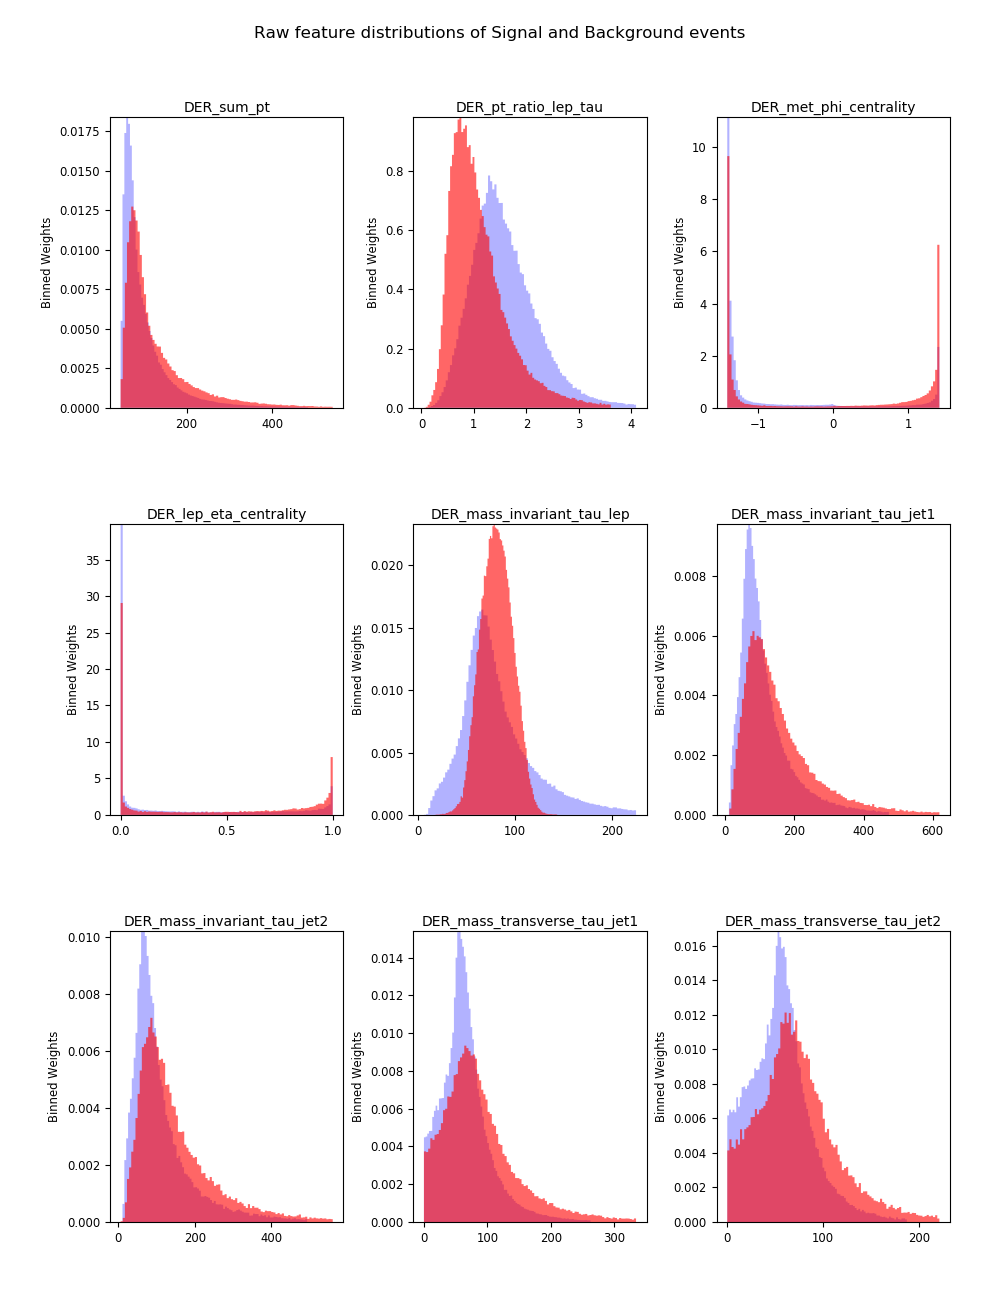
\includegraphics[width=\textwidth]{images/der_features2.png}
\caption[Raw feature distributions]{Raw feature distributions of signal (red) and background (blue) events depicting values on their true scale, further in order to make the histogram more representative we sum importance weights $w_{i}$ in each bin rather than count.}
\label{unscaled_features2}
\end{figure}

\subsection{Class overlap}

Fig. \ref{scatter1} and \ref{scatter2} provide a sense of the difficulty of the task of classifying background and signal events. Not only do the classes predominantly overlap, the densities of background and signal events captured by the importance weights $w_{i}$ attached to each event show that the signal is sparse and embedded in the background.  The features in the plots represented are from the more discriminatory derived features. 

\begin{figure}[ht]
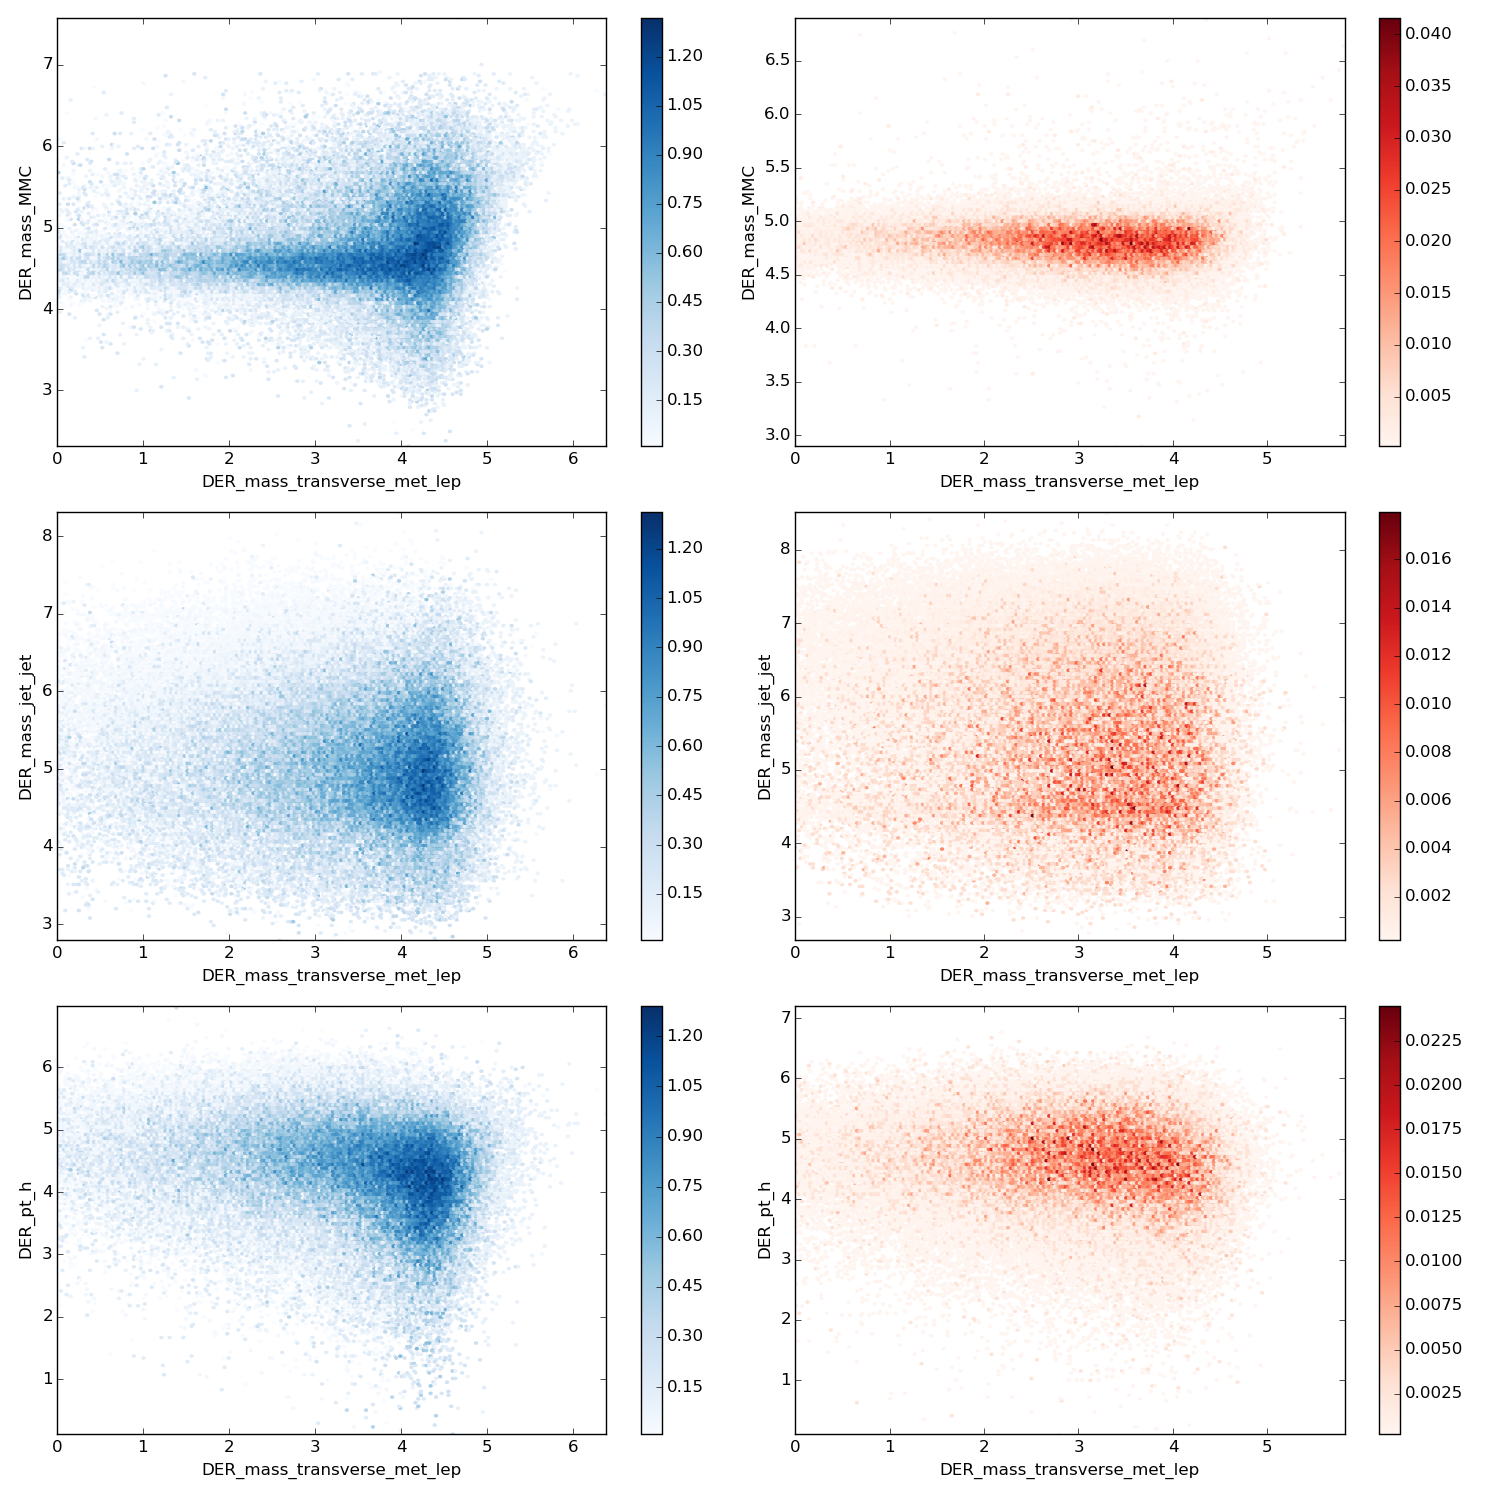
\includegraphics[width=\textwidth]{images/scatter1.png}
\caption{Density of weights of signal and background expressed in 2d space.}
\label{scatter1}
\end{figure}

\begin{figure}[ht]
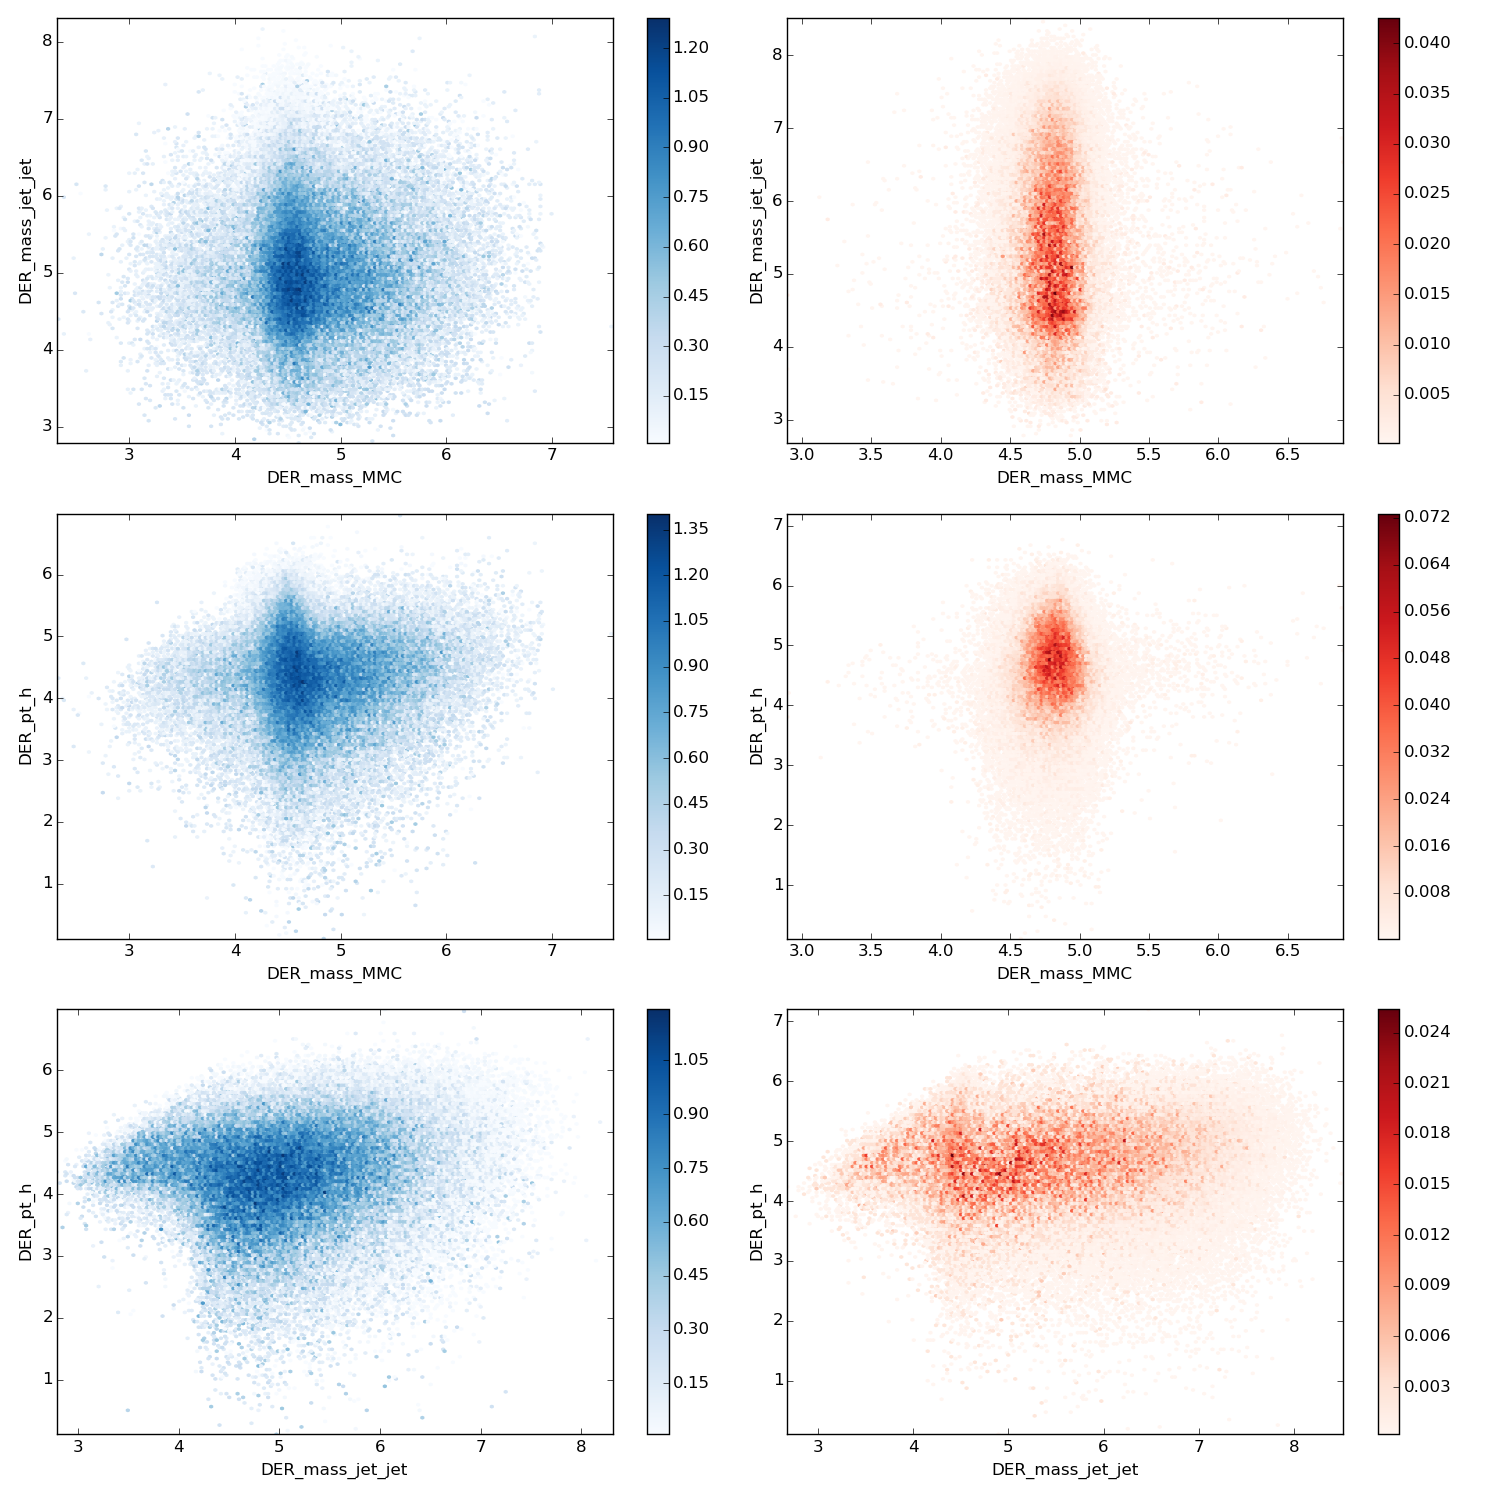
\includegraphics[width=\textwidth]{images/scatter2.png}
\caption{Density of weights of signal and background expressed in 2d space.}
\label{scatter2}
\end{figure}

\section{Tree ensembles}

The results presented in this section make use of the bagging principle used in random forests (RF) and extremely random trees (ET). The aim of this section is to establish a baseline performance for bagging methods using the primitive tree learner and provide some insight into the variations between random forests and extremely random trees. 

Intrinsic to the construction of the tree learner is the splitting principle, each tree in a RF uses a splitting rule based on a metric that scores all possible splits in a collection of features and then chooses the best split. On the other hand, extremely random trees do not use a splitting rule. They construct trees by choosing the best split from a set of random splits (see algorithm \ref{randomsplits}). This attribute of extremely random trees make them less accurate than random forests but much faster. Fig. \ref{tree_correlation} and \ref{et_tree_correlation} depicts the correlation between trees in a RF and ET model. ET trees are visibly less correlated than RF trees. The diagonal entries indicate the correlation of a tree output with itself. 

\begin{figure}[h]
\centering
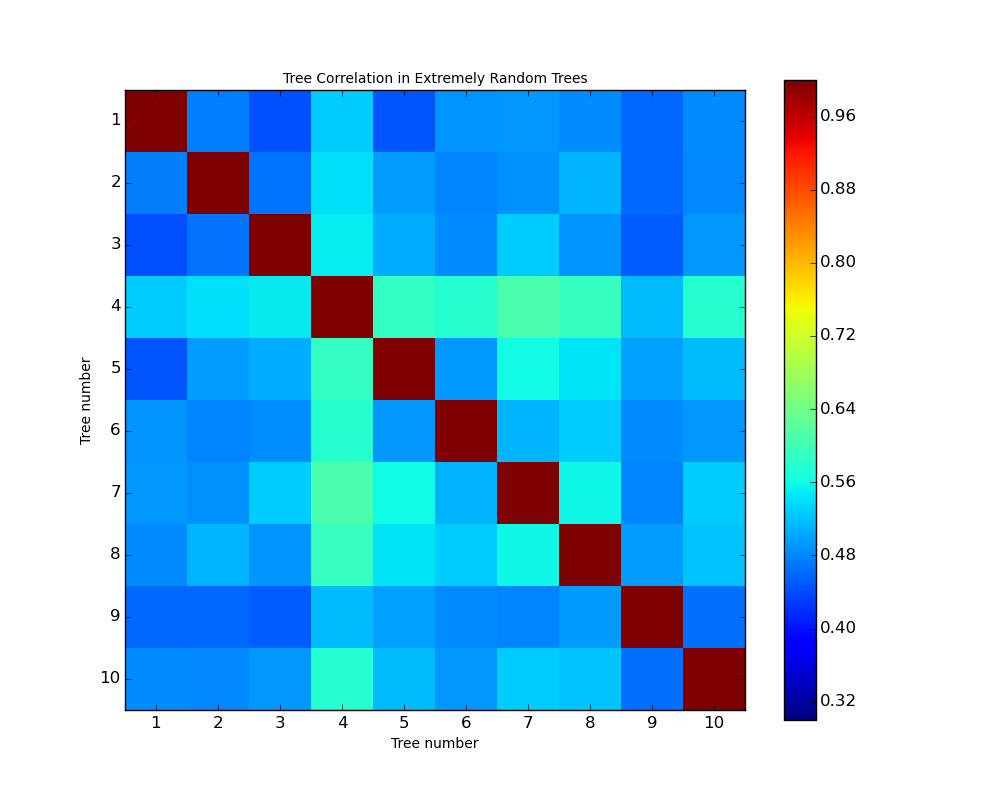
\includegraphics[scale=0.5]{images/ET_tree_correlation.png}
\caption{Correlation between tree outputs under the ET tree ensemble.}
\label{tree_correlation}
\end{figure}

\begin{figure}[h]
\centering
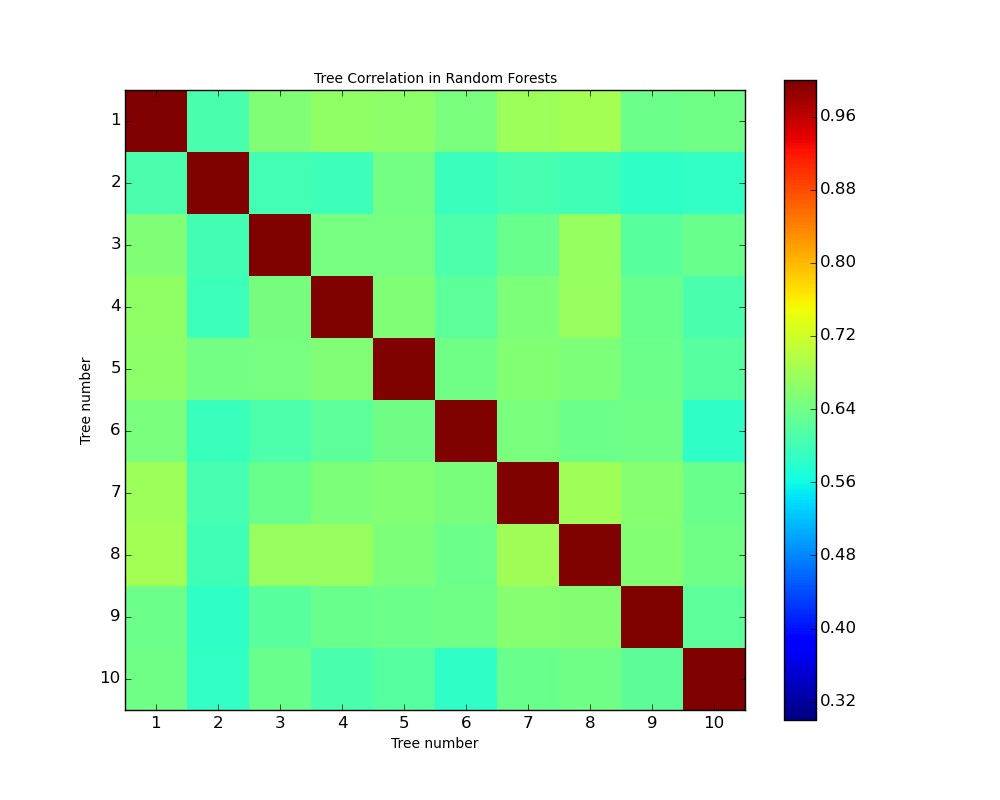
\includegraphics[scale=0.5]{images/RF_tree_correlation.png}
\caption{Correlation between tree outputs under the RF tree ensemble.}
\label{et_tree_correlation}
\end{figure}

Figure \ref{tree_num_features} shows the density of the balanced classification error on a grid of two parameters. The parameters here are the \textit{Max depth} and \textit{Max features}. The former refers to the maximum allowed depth of a tree and the latter refers to the maximum features considered to split on at each node. The magnitude of change in the balanced classification error is small due to the magnitude of the balanced weights (see fig. \ref{bweights}). A 0.001 difference in the balanced classification error amounts to on average 100 misclassified events. An interesting observation is that the tree ensembles saturate at 100 primitive learners and increasing the number of learners to 200 leads to a deterioration in error. %The same effect is a lot more muted in fig. \ref{depth_features}. The error seems to go down with higher depth and features. 


\begin{figure}[h]
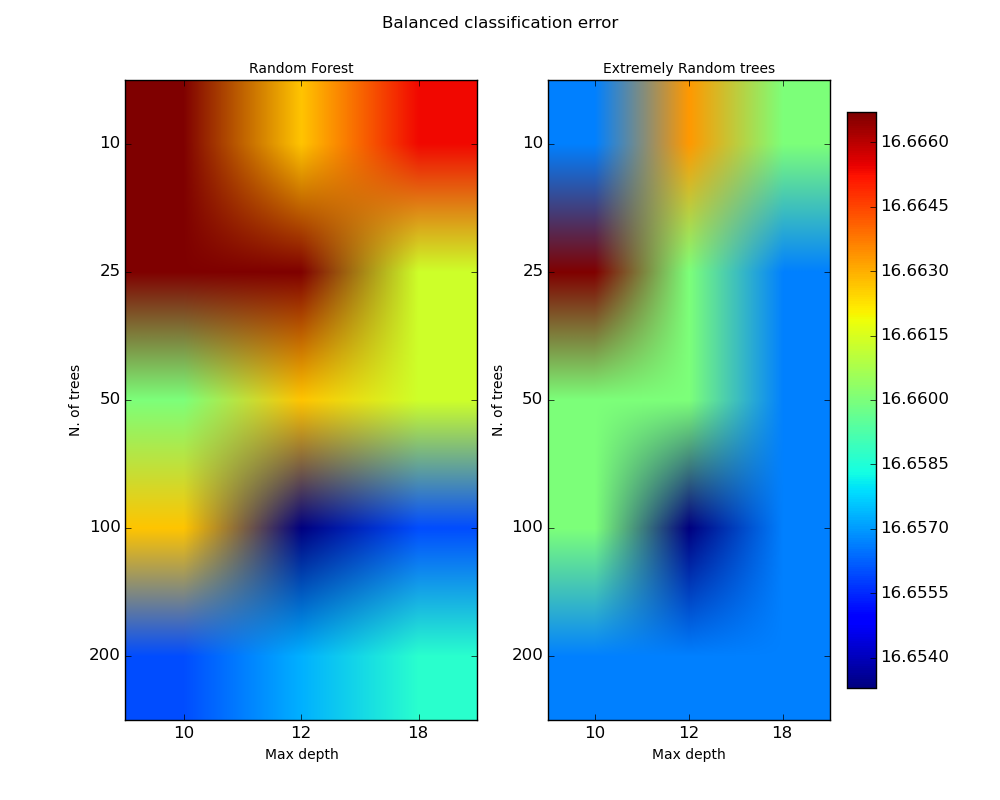
\includegraphics[scale=0.6]{images/Grid_error_depth_trees_rf_et.png}
\caption{Density of balanced classification error for tree ensembles - Max depth vs. number of trees}
\label{tree_num_features}
\end{figure}

The significance curves of RF and ET models are depicted in section \ref{sig} below. The next section presents results on the workings and behaviour of two meta-ensembles and highlights some important differences which make one more markedly suited to the classification task than the other. 
  
\section{Meta Ensembles}

In this section we analyse the results of two models on the Higgs dataset - boosted random forests (BRF) and boosted extremely random trees (BXT). As the name suggests each model works on the principle of boosting, but uses different base learners. As opposed to simple BDTs which boost a single decision tree, in BRFs and BXTs we boost a tree ensemble. An automated parameter search for the right parameters of such models is hard due to the combinatorial explosion in the parameter space. Instead the approach followed here is to look for convergence of the ensemble effect with respect to the AMS ($\sigma$).  We take our cue from the optimization in the earlier section where we analysed the performance and behaviour of random forests (RF) and extremely randomized trees (ET). These models are the base learners in the meta ensemble.  

\subsection{De-construction of Boosting}

In this section we analyse the effect that boosting has on the discriminant scoring function. The shape of the distribution of the discriminant score is critical to the selection of a pure selection region. Distributions which are spread out and fat-tailed indicate low confidence in scoring and tend to give poorer AMS scores. In figures \ref{staged} we observe the evolution of the discriminant score distribution at successive levels of boosting. We can notice how the incremental gains from boosting fall as the number of stages increases. This indicates some level of saturation in the models ability to predict more samples correctly than it already has in the previous stages. The distributions growing more peaked indicate greater confidence in the predicted scores.  
 
\begin{figure}[h]
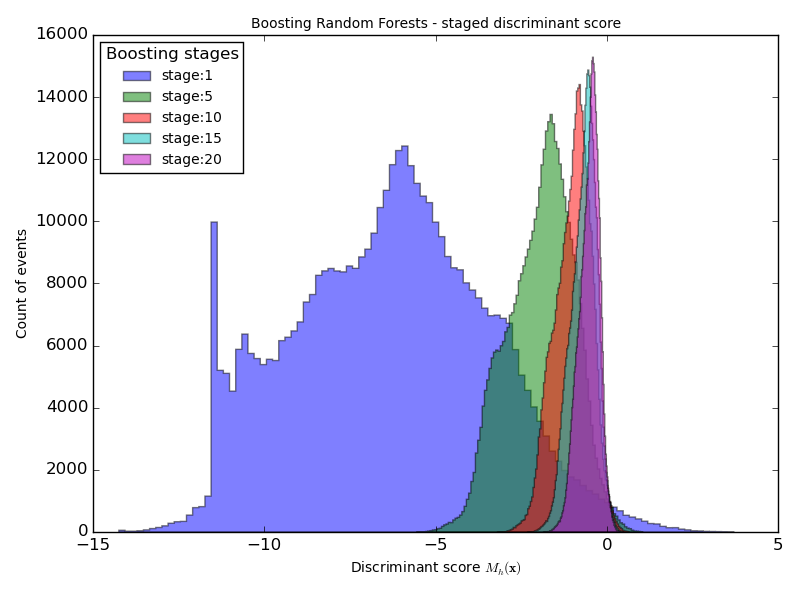
\includegraphics[width=\textwidth]{images/brf__staged.png}
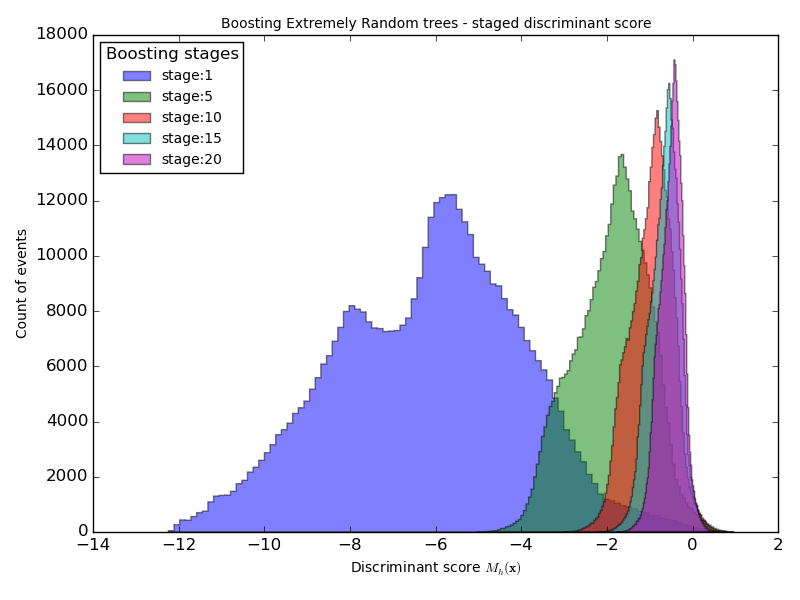
\includegraphics[width=\textwidth]{images/bxt__staged.png}
\caption[Evolution of discriminant score in BRF and BXT.]{Apart from the noticeable spike in the distribution of BRFs which results from a large number of samples getting an identical score, we can notice that the BRFs in stage one have a thicker right tail as opposed to the one of BXTs.}
\label{staged}
\end{figure} 

Since the AMS objective is tied to importance weights of each sample, it is often instructive to look at the staged distributions by contribution of weight of events in each bin (of the histogram). In figures \ref{staged_weighted} we represent this weighted score distribution in stages.  

\begin{figure}
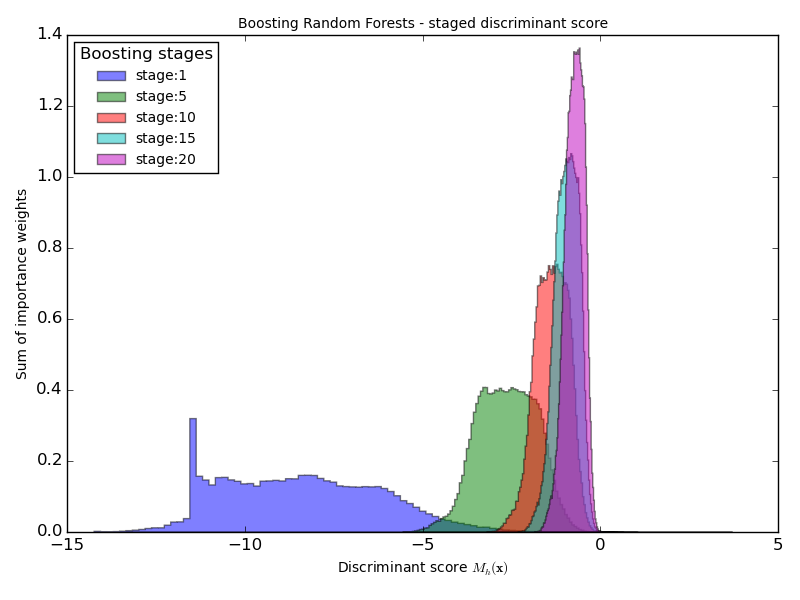
\includegraphics[width=\textwidth]{images/brf_weighted_staged.png}
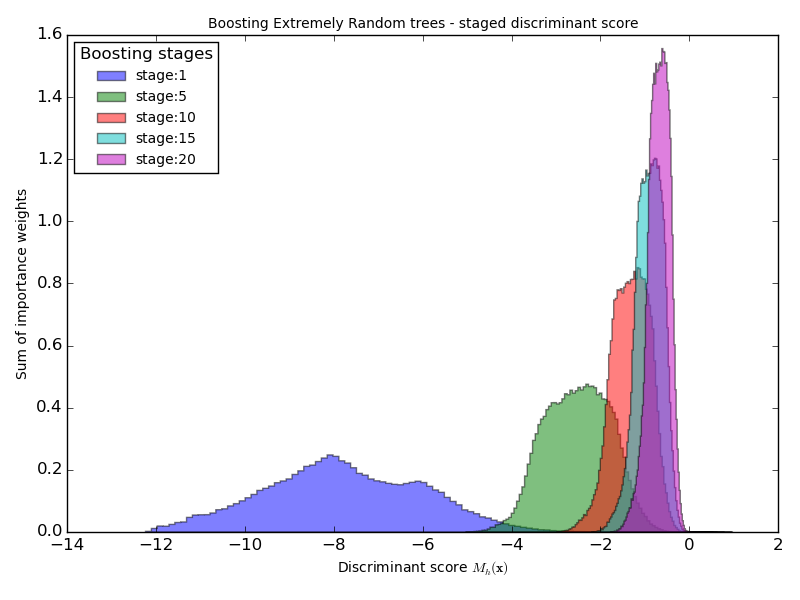
\includegraphics[width=\textwidth]{images/bxt_weighted_staged.png}
\caption[Evolution of weighted discriminant score in BRF and BXT]{The spike in events in the BRF score distribution is translated to a spike in the weights in the same region. At stage 20, the BXT model has a visibly higher peak than the BRF model.}
\label{staged_weighted}
\end{figure}

In figures \ref{brf_staged_weighted_bi} and \ref{bxt_staged_weighted_bi} we observe the weighted distribution of the discriminant score bifurcated by class. This is useful as it points to the region of overlap in the scores of signal and background events. The vertical red line indicates a typical cut (at the 85th percentile) that determines the selection region. The background events which lie on the right hand side of this cut are the false positives and directly impact the AMS $(\sigma)$. Boosting at a fundamental level targets the overlap between signal and background events successively. This is contrast to complex single stage classifiers that do not target the overlap issue per se, their effectiveness is mainly tied to the creation of complex decision boundaries in higher dimensional spaces. 

\begin{sidewaysfigure}
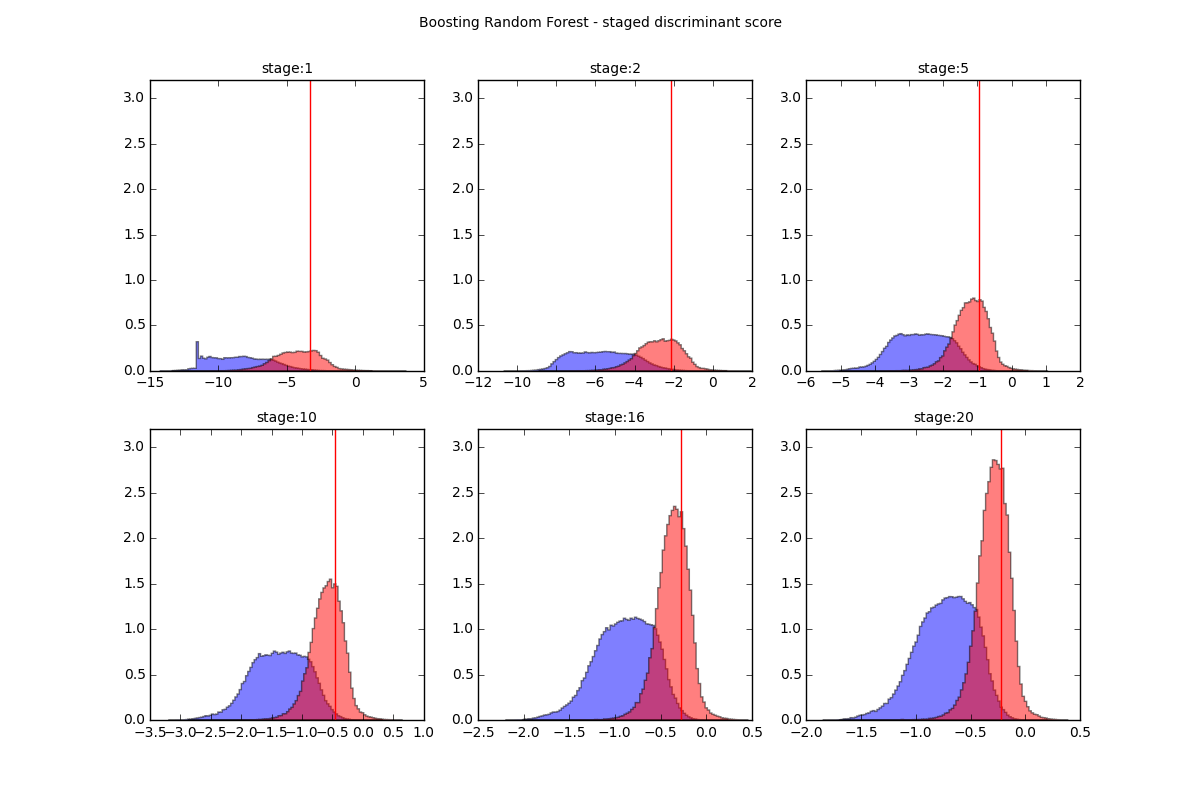
\includegraphics[scale=0.7]{images/brf_staged_bi.png}
\caption[Evolution of weighted discriminant score in BRF.]{Event which lie on the right hand side of this cut determine the selection region.}  
\label{brf_staged_weighted_bi}
\end{sidewaysfigure}

\begin{sidewaysfigure}
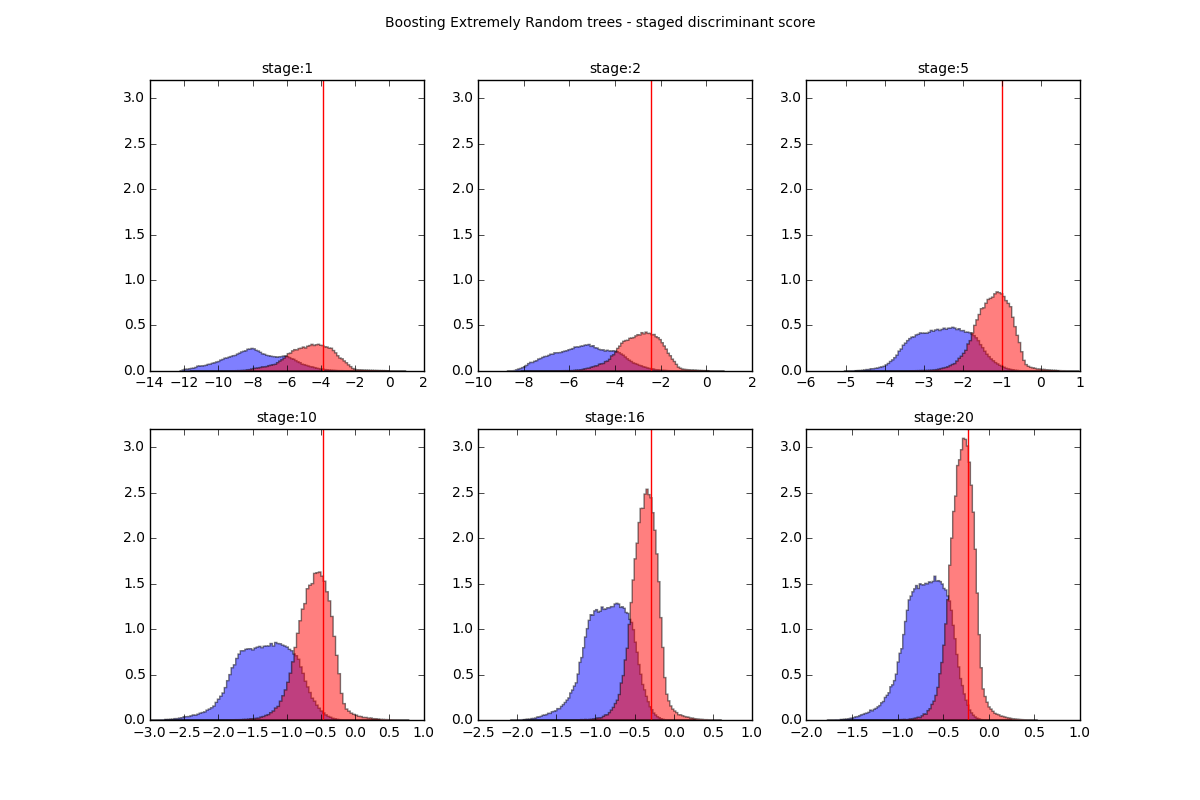
\includegraphics[scale=0.7]{images/bxt_staged_bi.png}
\caption{Evolution of weighted discriminant score in BXT.}
\label{bxt_staged_weighted_bi}
\end{sidewaysfigure}

From figures \ref{brf_staged_weighted_bi} and \ref{bxt_staged_weighted_bi} we see the narrowing of the width of the discriminant function but it is not clear if the actual count of false positives is going down in successive stages. Figure \ref{fp_evolve} depicts this information for both the models. Both the count and sum across weights of false positives ($\hat{b}$) drop with number of stages. In terms of count, it seems like both the models perform equally well however, in terms of the importance weights the models diverge after around 5 rounds of boosting. While the BRF is more effective in earlier stages at weeding out the false positives, its effectiveness saturates rapidly after round 5. The BXT model exhibits a slow and consistent decline in the weighted false positives. After 20 rounds, it is evident that BXT the selection region has fewer false positives than the BRF model.   

\begin{figure}
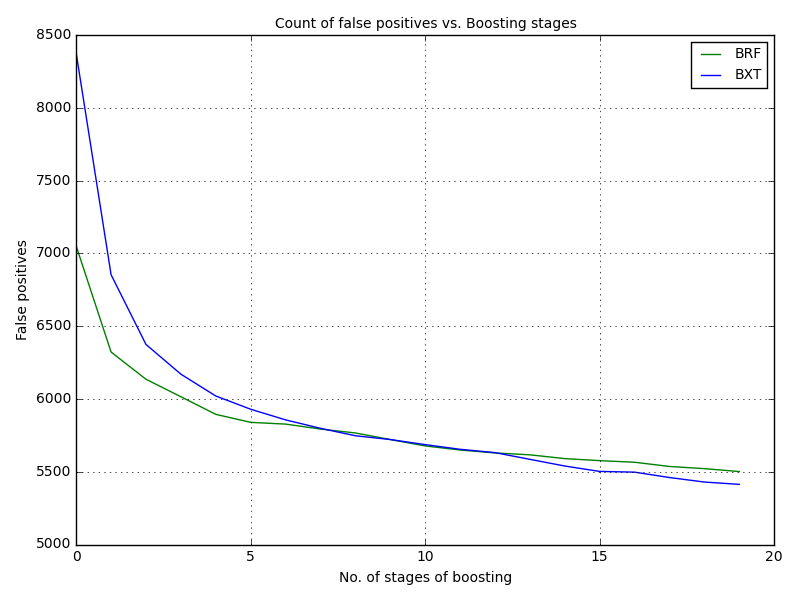
\includegraphics[width=\textwidth]{images/fp_counts.png}
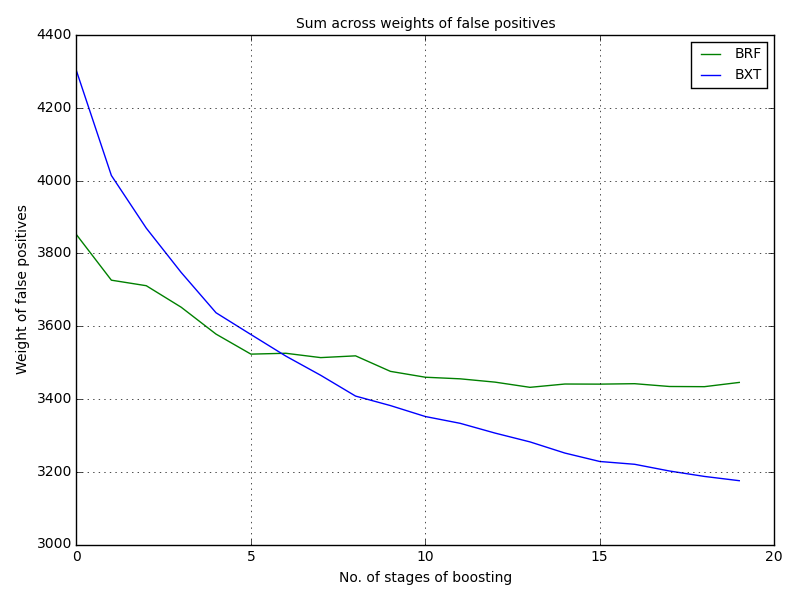
\includegraphics[width=\textwidth]{images/fp_weights.png}
\caption{Count and weights of false positives in the selection region for classifiers - BRF and BXT}
\label{fp_evolve}
\end{figure}

\subsection{Tree correlations}

Correlation between trees is fundamental to the effectiveness of the BXT model. Figure \ref{boosted_correlations} depicts the correlation between 100 primitive trees picked at random from 
the 2000 trees that comprise the final stage BRF and BXT model (20 stages of boosting $\times$ 100 trees in each tree ensemble). The higher level of de-correlation between the outputs of BXT versus the BRF indicate two critical aspects:

\begin{itemize}
\item BXT creates more diverse tree ensembles than BRF, diversity in the context of classification means that each tree ensemble is good at predicting different events. Diversity in the ensembles gives the model access to predicting a larger number of points correctly. The BRF trees are more correlated in their predictions, saturating their predictive ability.
\item BXT is able to benefit from more rounds of boosting than BRF, as we saw in fig. \ref{fp_evolve}. The main reason for this is that the BRF model is a strong predictor and boosting on strong predictors is not as beneficial as boosting on moderately weak predictors. 
\end{itemize} 
 
\begin{figure}
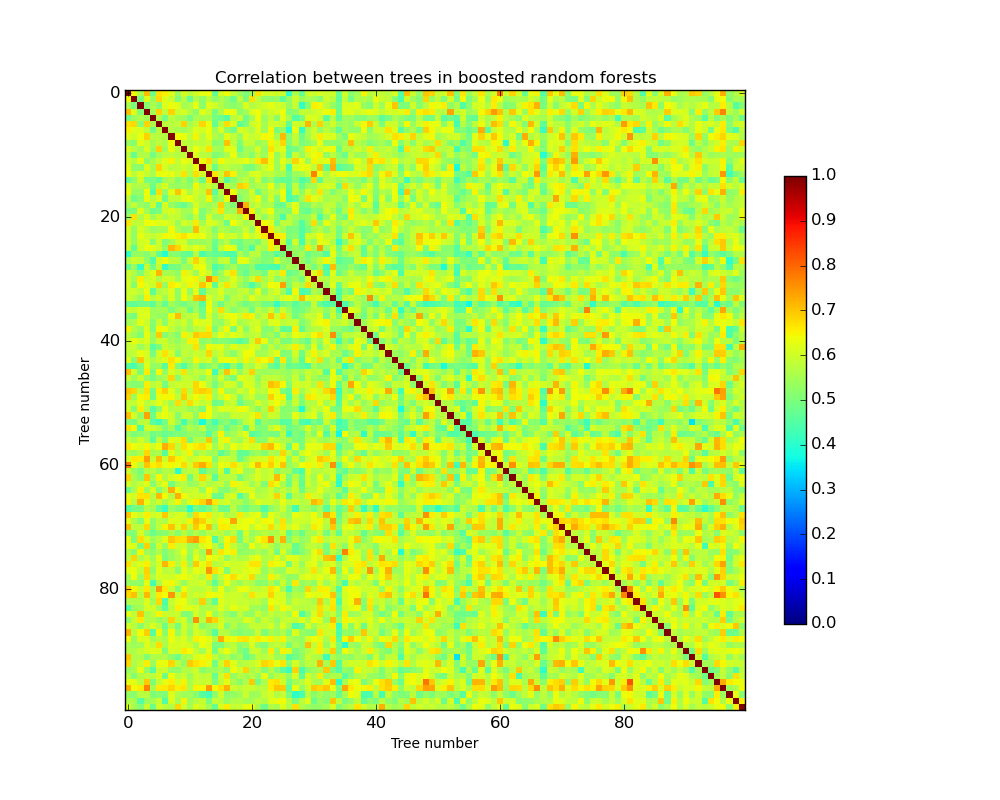
\includegraphics[width=\textwidth]{images/BRF_tree_correlation.png}
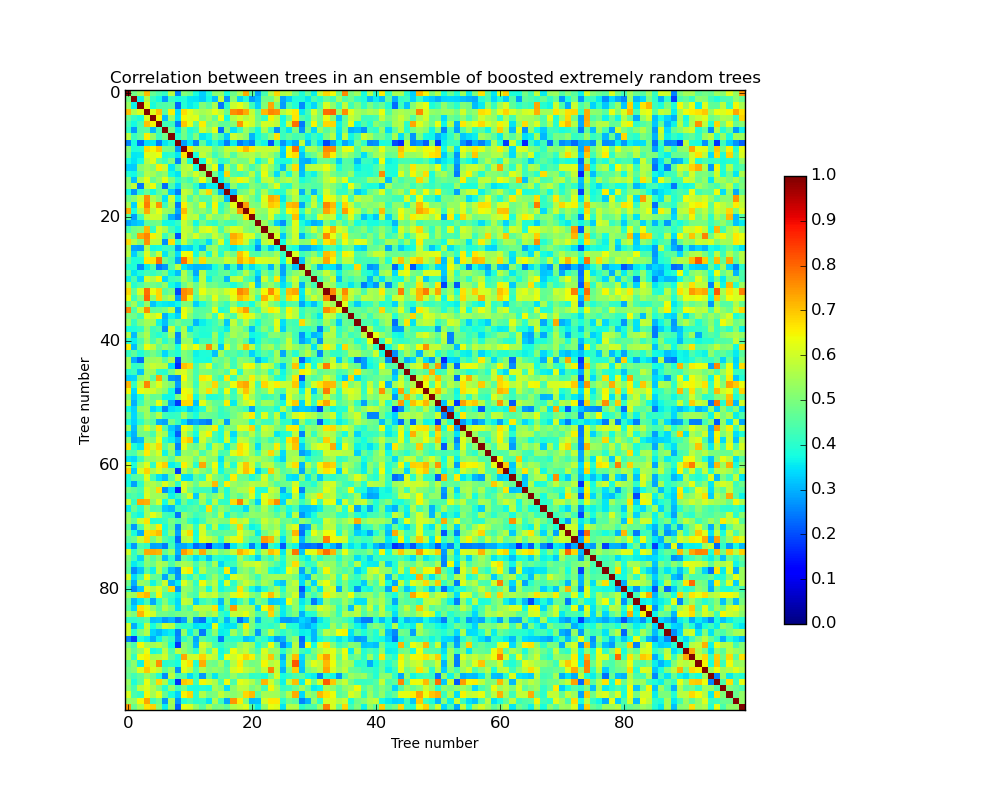
\includegraphics[width=\textwidth]{images/BXT_tree_correlation.png}
\caption{Correlation between trees in BRF and BXT.}
\label{boosted_correlations}
\end{figure}

\section{Significance Curves \texorpdfstring{$(\sigma)$}{}}
\label{sig}

For the tree ensembles proposed in this study, the AMS ($\sigma$) is the definitive measure of performance. In this section we summarize the results of the AMS objective introduced in detail in chapter \ref{formal}. The AMS ($\sigma$) is computed using the events in the selection region of a classifier. The AMS is essentially the ratio $\hat{s}/\sqrt{\hat{b}}$ where $\hat{s}$ and $\hat{b}$ are the sum across importance weights of signal and background events in the selection region (see \ref{unbiased}). The exact mathematical form used in the figures in this section is, 

\begin{equation}
\sqrt{2((\hat{s} + \hat{b})\ln(1 + \frac{\hat{s}}{\hat{b}})-\hat{s})} 
\end{equation} 

The AMS ($\sigma$) appears on the $y$ axis. In order to facilitate comparison with the leading solution to the $H \rightarrow \tau{+}\tau^{-}$ classification problem presented in the ATLAS Higgs dataset, each plot has a horizontal red line which indicates the leading published score on this dataset.\footnote{This was the winning score on the ATLAS Kaggle machine learning competition held in 2014.} 

\subsection{Single Ensembles}

Fig. \ref{cluster} depicts the evolving AMS curves for a random forest ensemble (RF) and the extremely random trees ensemble (ET). The curves are evolving with respect to the number of primitive tree learners in the ensemble. This figure depicts the `bagging' effect in the context of inseparable classes. Aggregating a large number of primitive learners improves the overall performance. Averaging predictions reduces the variance of the predictions but increases the bias, the overall classification error is attributed to both - variance and bias. This was discussed in chapter \ref{performance}. The effect we see here is that the improvement in error due to reduction in variance is large enough to offset the increase in bias due to averaging.  

\begin{figure}
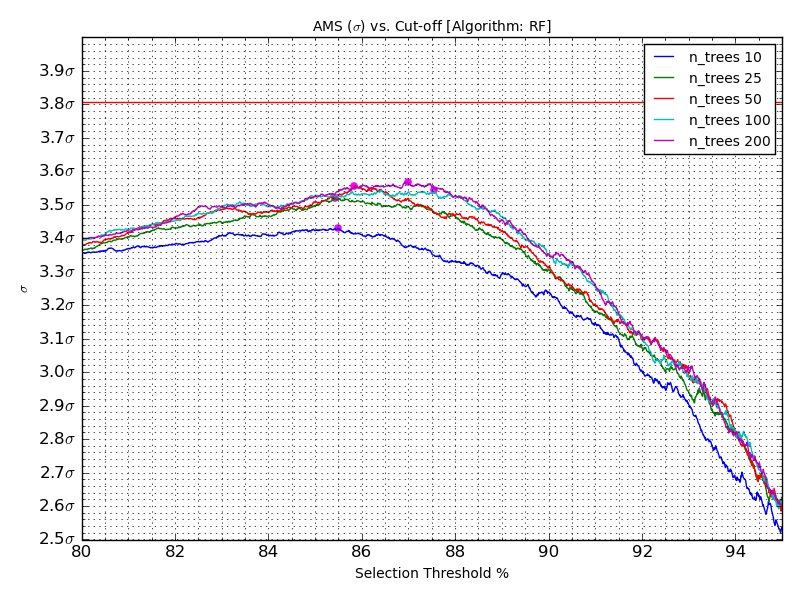
\includegraphics[width=\textwidth]{images/AMS_Curve_RF_Cluster.png}
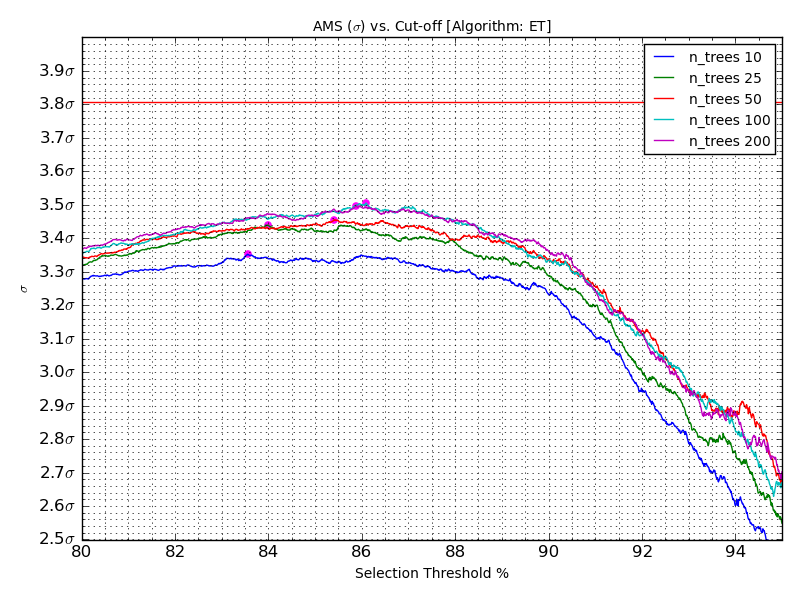
\includegraphics[width=\textwidth]{images/AMS_Curve_ET_Cluster.png}
\caption[AMS curves corresponding to increasing number of trees.]{We can observe the progression of curves in the ET model more clearly than in the RF model.}
\label{cluster}
\end{figure}

It is important to note that the individual RF model is slightly better than the individual ET model at all levels. In order to put the significance curves of each algorithm into perspective, the figure \ref{ams_et_rf} shows the evolution of the best significance ($\sigma$) with respect to the number of trees in the ensemble for each algorithm. It is essentially a plot of the magenta dots ({\color{magenta}\small{$\bullet$}}) on each  of the curves in fig. \ref{cluster}.

\begin{figure}
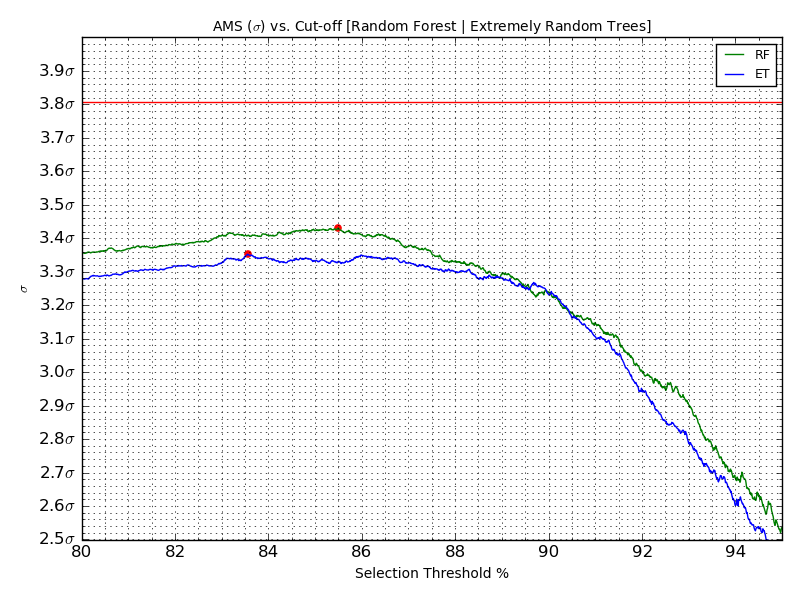
\includegraphics[width=\textwidth]{images/AMS_Curve_ET_RF.png}
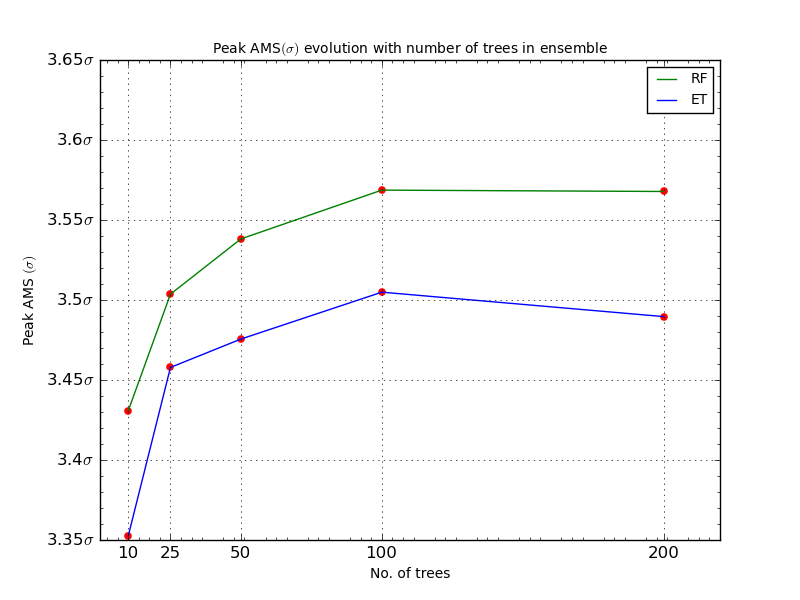
\includegraphics[width=\textwidth]{images/Peak_AMS_Evolution.png}
\caption{Comparitive performance of AMS on the RF and ET model}
\label{ams_et_rf}
\end{figure}

\subsection{Boosted Ensembles}

This section depicts the significance curves of boosted ensembles, each tree ensemble goes through several stages of boosting where the misclassified samples from the previous stages are over weighted. While a single extremely random trees classifier (ET) falls short of performing as well as a random forest, it is clear that in the boosted incarnation of the ensembles, BXTs steal an edge over the forests. In fig. \ref{ams_boosting} we observe a marked progression of curves in the BXT model in response to boosting while in the BRF model, the effect is more muted. 

\begin{figure}
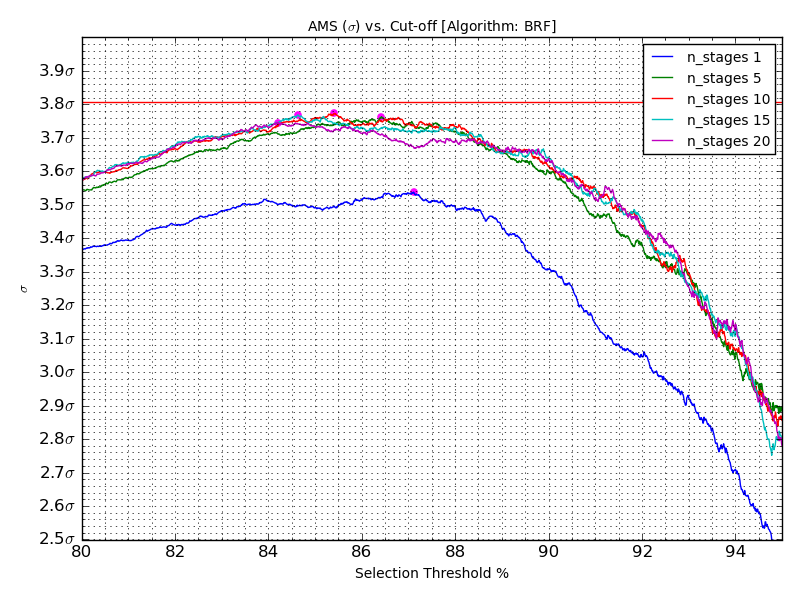
\includegraphics[width=\textwidth]{images/AMS_Curve_BRF_Cluster.png}
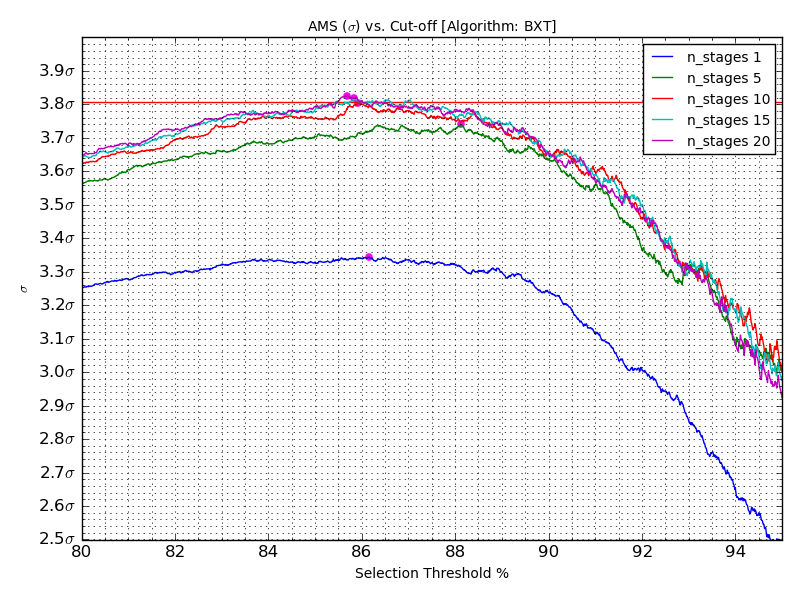
\includegraphics[width=\textwidth]{images/AMS_Curve_BXT_Cluster.png}
\caption{AMS curves at $n$ stages of boosting}
\label{ams_boosting}
\end{figure}

Figure \ref{ams_brf_bxt} depicts the AMS performance at the end of 20 rounds of boosting tree ensembles. BXT with extremely random trees as primitive learners give a consistently better AMS ($\sigma$) value across a range of selection thresholds. In order to facilitate a comparison between the two models, they use the same number of primitive trees (no. of trees = 100) in each stage of boosting. The AMS for the BXT model is comparable to the leading solution on this dataset. The evolution of the peak AMS gives further insight into the behaviour of the models. The peak AMS of the BRF model saturates within a few stages of boosting indicating that further stages do not add any value to the model, the same behaviour is seen in the BXT model but at a much later stage of boosting.   

\begin{figure}
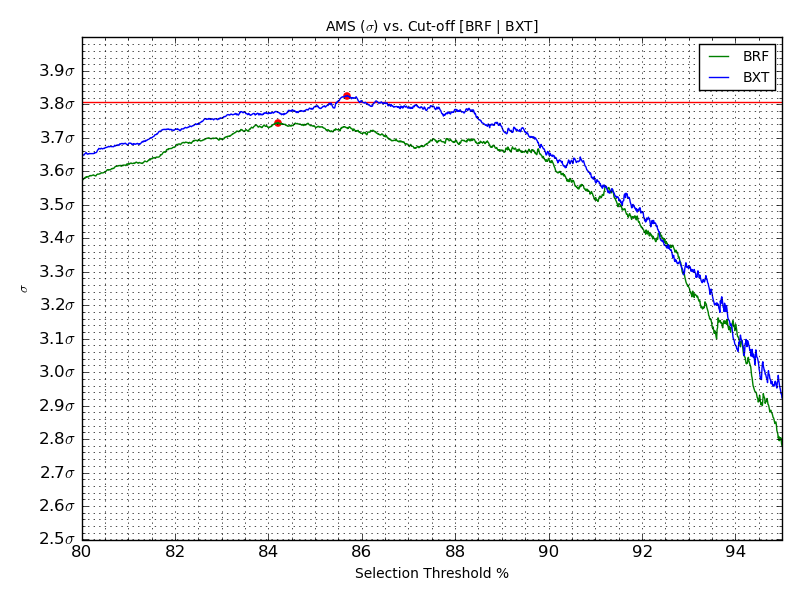
\includegraphics[width=\textwidth]{images/AMS_Curve_BXT_BRF.png}
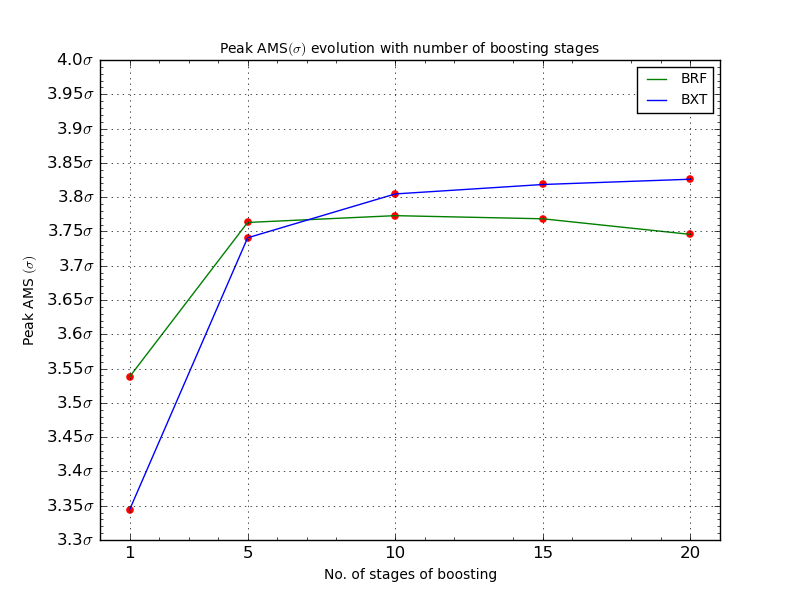
\includegraphics[width=\textwidth]{images/Peak_AMS_Evolution_BRF_BXT.png}
\caption{Best AMS curves for boosted forests (BRF) and boosted extremely randomized trees (BXT).}
\label{ams_brf_bxt}
\end{figure}

\section{Summary of Tree Ensembles}

The table \ref{treeams} summarizes the performances of tree ensembles. All results reported are based on the test dataset of 450K events. 

\begin{center}
\begin{table}[H]
\resizebox{\textwidth}{!}{
\begin{tabular}{l|c|c|c|c}
Learning Algorithm & Selection Region & False Positives & AMS at 85th percentile ($\sigma$) & Primitive Learners\\
\toprule
Random Forest (RF)  & 67632 & 7132 & 3.42294$\sigma$ & 100\\
Extremely Random Trees (ET)  & 67766 & 8106 & 3.33157$\sigma$ & 100 \\
Boosted Random Forests (BRF)  & 66789 & 5501& 3.73311$\sigma$ & 20 $\times$ 100\\
Boosted Extremely Random Trees (BXT)  & 66876 & 5413 & 3.79361$\sigma$ & 20 $\times$ 100\\
\end{tabular}}
\caption{Performance metrics of tree ensembles}
\label{treeams}
\end{table}
\end{center}

The BXT ensemble shows it is possible to leverage the performance of blazingly fast primitive tree learners for complex classification tasks where the data is inseparable and overlapping. Primitive trees have a computational edge over other classifiers albeit they give simple decision boundaries compared to more powerful classifiers like kernel support vector machine and neural nets. However, in several problems trees have shown to claw back the loss in accuracy if enough of them are harnessed in a meta approach. The next section discusses the computational elements of tree ensembles and draws some perspectives by comparing to the leading solution.  

\section{Computing}

The architecture of the meta algorithm BXT imposes some level of serial execution. Since the training occurs iteratively in independent stages the pipeline for training and testing essentially work in a serial fashion. 

Within each stage of training we use a randomized forest as a base learner, this algorithm works on the principle of bagging which is an apt candidate for parallel execution. In bagging, the training of each bootstrap sample is conducted independently, hence they can be generated in parallel. 

The size and dimensionality of the dataset were relatively tractable and did not prove to be computational bottlenecks. The full dataset comprised of 800K samples and 30 features, 5 redundant features were dropped and 9 additional features were added during preprocessing leaving the original size relatively unchanged. An advantage of tree learners is their training speed relative to models like neural networks which are much slower to train. Python provides an efficient version of the CART algortihm in its \texttt{scikit-learn} package which was used to train the primitive learners in the ensemble.  
 
The table \ref{treetimes} summarizes the training speed of the algorithms alongside their implementation details.

\begin{table}[H]
\resizebox{\textwidth}{!}{
\begin{tabular}{l|c|c|c|c|l}
Learning Algorithm & Training speed & Learning Stages & No. of Trees & Tree Construction & Machine specs \\
\toprule
Single Decision Tree  & 4.77 sec. & 1 & 1 & Serial &  \rdelim\}{6}{20pt}[\parbox{18.5mm}{Intel Xeon (R) CPU \\ 3.10GHz x 4}] \\
Boosted Single decision trees (BDT) & 45.28 sec. & 30 & 1 & Serial  \\
Random Forest (RF) & 70 sec. & 1 & 30 &  Parallel &  \\
Extremely Random trees (ET) & 26 sec. & 1 & 30 &  Parallel & \\
Boosted Random Forests (BRF) & 1025 sec. &  20 & 100 & Parallel &   \\
Boosted Extremely Random Trees (BXT) & 983 sec. & 20 & 100 & Parallel &  \\
\end{tabular}}
\caption{Runtime of tree ensembles on a single CPU 4-core machine}
\label{treetimes}
\end{table}

In the table we choose the same number of trees for the bagged models (RF, ET) as the number of stages in BDT to facilitate a comparison between the two from a computational viewpoint. The computational load of training a single tree 30 times (one time per stage for BDT) is identical to training 30 trees one time (bagged, RF and ET). Extremely random trees are faster than random forests as they by pass the search for the best split at each node of the primitive tree learner. The computational advantage coupled with a consistently higher AMS ($\sigma$) curve point to the effectiveness of the meta algorithm in the Higgs classification task. Gabor Melis (the owner of the lead solution) trained his ensemble of neural networks on a GTX Titan GPU where training a single 3-layer network took 10 minutes. As a comparison the solution provided in this thesis runs on a 4-core CPU machine and the entire model trains in under 20 mins. The boosted extremely random trees (BXT) algorithm proposed in this thesis achieves an AMS score of 3.79361$\sigma$ at the 85th percentile cut-off.

Fig. \ref{runtime} depicts the training speed of ETs versus RFs, they grow linearly in the number of trees in the ensemble.  

\begin{figure}
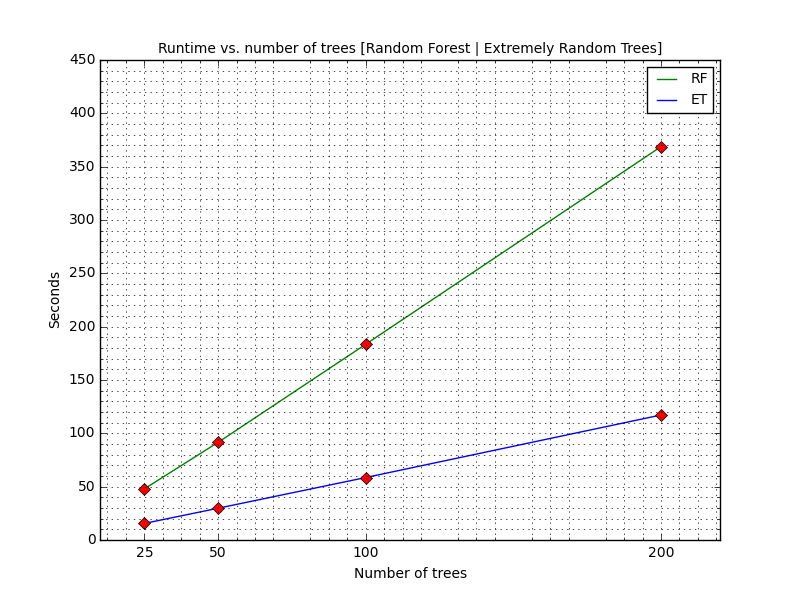
\includegraphics[width=\textwidth]{images/Runtime_evolution_RF_ET.png}
\caption{Training Speed}
\label{runtime}
\end{figure} 

\section{Complexity}

In this section we briefly summarise the computational complexity of the learning algorithms used in this thesis. We present this information using the `Big $\mathcal{O}$ notation' which in this context describes how the algorithm scales to changes in the input size. Mathematically, it provides an upper bound for the growth of a function ignoring lower order terms. 

\begin{equation}
f(n) = n^{4} + 4n^{3} + n^{2} + 7 = \mathcal{O}(n^{4}) \textrm{ as } n \rightarrow \infty 
\end{equation}

\subsection{Single Decision Tree}

The cost of constructing a binary tree using $n$ samples and 1 feature vector is $\mathcal{O}(nlog_{2}(n))$. In the presence of $s$ features, splitting at each node requires searching through $\mathcal{O}(s)$ features to find the best split, this amounts to a total complexity of $\mathcal{O}(sn\log_{2}(n))$. In order to query a single data point (pass an unseen data point down a tree until it reaches a leaf), the complexity is $\mathcal{O}(\log_{2}(n))$. 

\subsection{Tree ensemble}

In a random forest, where we specify the number of trees, say $M$ trees, the complexity is $\mathcal{O}(Msn\log_{2}(n))$. However, this is not exact as in a random forest, each split considers a random subset of features and this random selection of features adds an additional overhead.  

The $\mathcal{O}(Msn\log_{2}(n))$ complexity is worst-case assuming that the depth of the tree is going to be $\mathcal{O}(\log_{2}(n))$. In most cases the stopping criterion causes the tree to terminate much before it attains its maximum depth and hence this upper bound is rarely reached. For instance, if we set a criterion for the minimum number of samples required for a node split to be 500, nodes with less than 500 samples would convert to leaves and stop growing on that branch. Rules like these prune the unbounded growth of a tree to its maximum achievable depth, they serve as over fitting control. Trees fitted to a training dataset that are allowed to grow to their maximum depth are rarely useful for prediction on new samples as they over fit the training dataset. If the depth of each tree is specified as a parameter before training, the tree stops growing when it achieves the pre-specified depth. In this case the worst case complexity is simplified to $\mathcal{O}(Msnd)$ where $d$ is the pre-specified tree depth.

In order to query a single data point on a random forest with $M$ trees of depth $\log_{2}(n)$, the complexity is $\mathcal{O}(M\log_{2}(n))$. With $M$ trees of depth $d$, it becomes $\mathcal{O}(Md)$.

\subsection{Boosted ensemble}

The complexity of a boosting algorithm where the complexity of the underlying base learner, say $T$ is $\mathcal{O}(T)$ is $\mathcal{O}(NT)$ where $N$ is the number of rounds of boosting. The dependence is trivially linear as in each stage the cost is $\mathcal{O}(T)$ and with $N$ stages, it is $\mathcal{O}(NT)$. Where T is a random forest with $M$ trees, the cost of boosting $N$ random forests is $\mathcal{O}(NMsn\log_{2}(n))$. The cost of querying a $N$ stage boosting algorithm with a random forest (of $M$ trees) as base learner is $\mathcal{O}(NM\log_{2}(n))$.  



 